\documentclass{sig-alternate}

\usepackage{epsfig}
\usepackage{subfigure}

\makeatletter
\def\@copyrightspace{\relax}
\makeatother

\title{Efficiency Simulation for Bus Traffic in Taipei City}
\numberofauthors{3}
\author{
 \alignauthor
 Tsung-Hsien Wen\\
 	\email{r00921033@ntu.edu.tw}
 \alignauthor
 Po-Chun Hsu\\
 	\email{r00921034@ntu.edu.tw}
% \alignauthor
% Heng Wang\\
% 	\email{r00944042@ntu.edu.tw}
 }
\begin{document}
\maketitle

\begin{abstract}
For newcomers in Taipei, the bus system there is hard to figure out since there are too many bus lines.
In addition, some of the lines are tortuous and make travellers spend much more time than expected.
Consequently, travelling by bus might be inefficient for those who are not experienced in taking bus in Taipei.
From another perspective, this kind of bus network is energy-consuming as well.
A chessboard-like bus network has been thought to be a solution to these problems for many years, although it has not been promoted successfully in Taipei.
We thus want to know whether a chessboard-like bus network works better in Taipei.
We set up a simulation to observe what are the pros and cons of a chessboard-like bus network and the current bus network.
We encoded a part of roads in Taipei into a graph.
Two types of agents, buses and clients, are placed in the simulation environment.
In order to simulate the behaviors of buses, we record the routes and intervals of buses from the Taipei e-bus website.
We also set up different scenario types to simulate client behaviors at different time points of a day.
The simulation results suggest that a chessboard-like bus network is more efficient in terms of the resource utilization.
Even though the data are still limited so real-world clients is hard to model, this simulation is an initial attempt to model the bus activities in Taipei and gives us some insight on future policies of public transportation.
\end{abstract}

\section{Introduction}
In Taipei City, which is the city with its total area around 271.7997 square kilometers, there are about 300 bus routes in operation in which the density is extremely high.
Several of them are long trajectory detours, which makes the bus management really hard to handle.
Due to the overfull bus routes, people living in Taipei City could have observed that many routes overlap with others and that sometimes bus jam occurs at a bus stop.
In addition, for those tortuous bus routes, buses travelers may spend more time hanging on the bus than the real value it really takes.
On the other hand, in the resource utilization efficiency point of view, the long and wind bus routes make the resource utilization very inefficient and hard to optimize.
The overlapped bus routes produce the redundancy of buses and thus make the  average passenger volume too small, which doesn't make the best benefit of each bus in operation.
Furthermore, since there're many long routes on the map which is based on the truth that the average bus run on the map in each particular time span is more than needed, these facts cost the government or companies need to spend more money on the investment of bus numbers rather the quality that really affects the experience of transportation.
These problems have existed and been noticed for many years.
Many people have tried to find out a better working bus system that brings the best of benefits into play in Taipei City.

A chessboard-like bus network has been thought to be a solution to the above problems.
In the late 1980s', an initial prototype of a chessboard-like bus network started to operate, but soon they became not that
Most of the routes are therefore not in operation now.
Nevertheless, in 2006, the the Commissioner of the Taipei City Department of Transportation tried to promote a new bus route network again.
Due to opposition from some frequent bus takers who did not transfers between buses and, more importantly, from the bus companies which had vested interests (about 15 bus companies are in operation), the new policy was not executed.
In 2010, Taipei City councilors hurried the government to promote the policy, but it is still the old system operated in Taipei City.

Despite that the problems of bus transportation is not only a engineering problem, we want to know whether a chessboard-like bus network is more efficient or more convenient than the current system in Taipei City theoretically.
The purpose of this project is to set up a simulation of behaviors of buses and clients and to observe what influences the efficiency of the bus traffic system.

\section{Data collection}
For our real-case simulation, we transform a map of part of Taipei City into a graph with roads as edges and intersections as nodes.
We need distances between each two nodes, current traffic information, stops of the bus routes and time intervals of the buses.
They are all available but are hard to fetch automatically.
To get these data, we have used the most powerful parser in the world!
We collect the road conditions from Google Map and the bus information from the website of Taipei Public Transportation Office manually.

We select an area of Taipei City as in Figure~\ref{fig:tpemap}.
We transform it into a graph as in Figure~\ref{fig:graphex}, where edges represent the roads in the area and nodes represent the intersection of the roads.
On the graph, we add the information of roads as in Figures~\ref{fig:node} and~\ref{fig:edge}.
We record the bus routes and intervals as in Figures~\ref{fig:bus}.

\begin{figure}
\centering
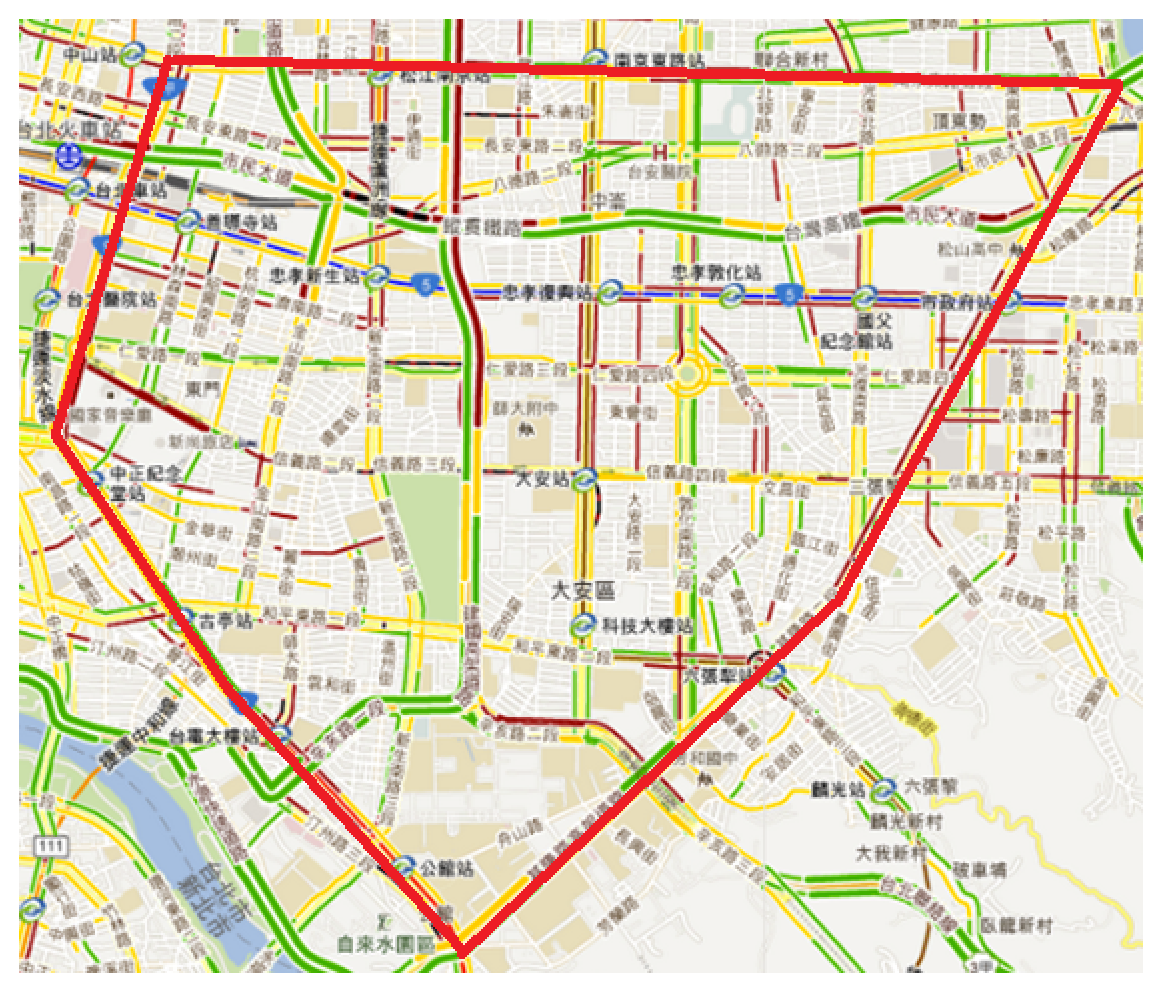
\includegraphics[height=2.5in, width=3.1in]{taipeimap.eps}
\caption{The framed area is transformed into the graph shown in Figure~\ref{fig:graphex}.}
\label{fig:tpemap}
\end{figure}

\begin{figure}
\centering
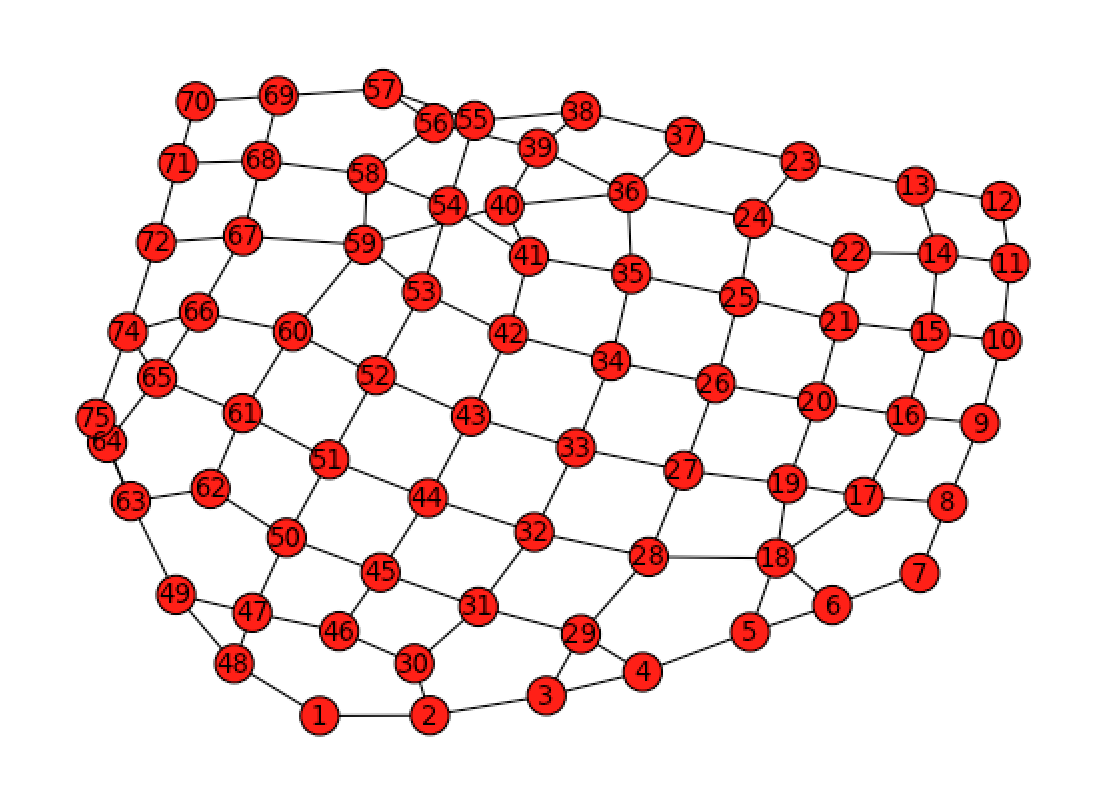
\includegraphics[height=2.2in, width=3.1in]{graphexample.eps}
\caption{In this graph, edges represent the roads and nodes represent the intersections.}
\label{fig:graphex}
\end{figure}

\begin{figure}
\centering
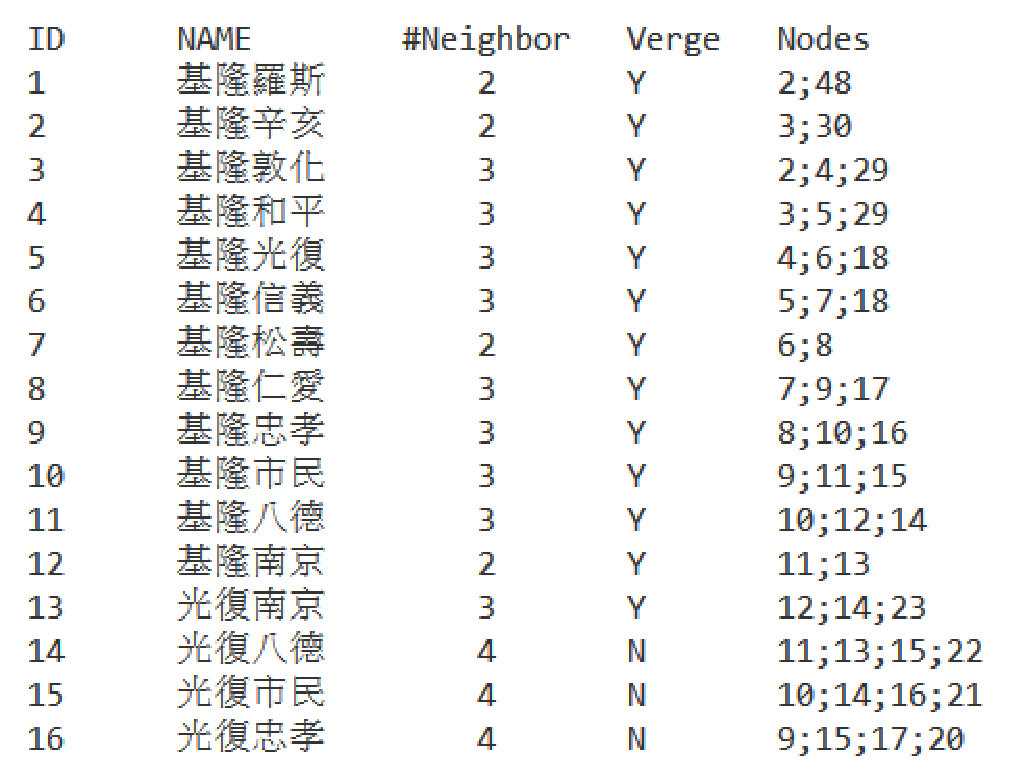
\includegraphics[height=2.4in, width=3.1in]{node.eps}
\caption{Part of the node information (totally 74 nodes). The entries for each node are its ID number, its name, its number of adjacent nodes, whether this node is on the verge, and its adjacent nodes.}
\label{fig:node}
\end{figure}

\begin{figure}
\centering
\subfigure[]{
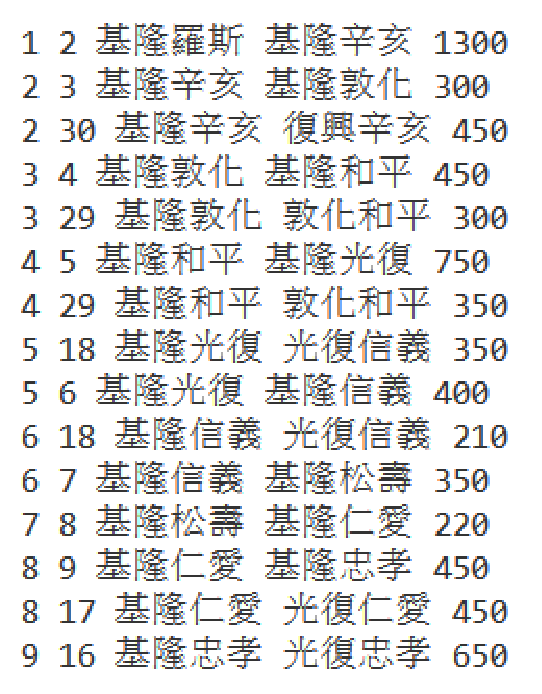
\includegraphics[height=1.5in, width=1.2in]{edge.eps}
\label{subfig:edge}
}
\subfigure[]{
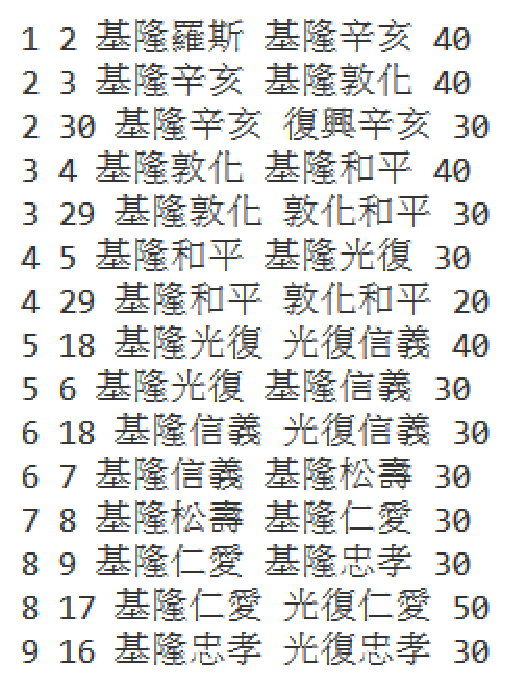
\includegraphics[height=1.5in, width=1.2in]{traffic.eps}
\label{subfig:traffic}
}
\caption{Figure~\ref{subfig:edge} is part of the edge information (totally 134 edges), where the entries for each edge are its two ends, the two ends' names, and the distance between the two ends; Figure~\ref{subfig:traffic} is part of the traffic conditions, where the
number in the last entry is the speed buses can drive at on the corresponding edge.}
\label{fig:edge}
\end{figure}

\begin{figure}
\centering
\subfigure[]{
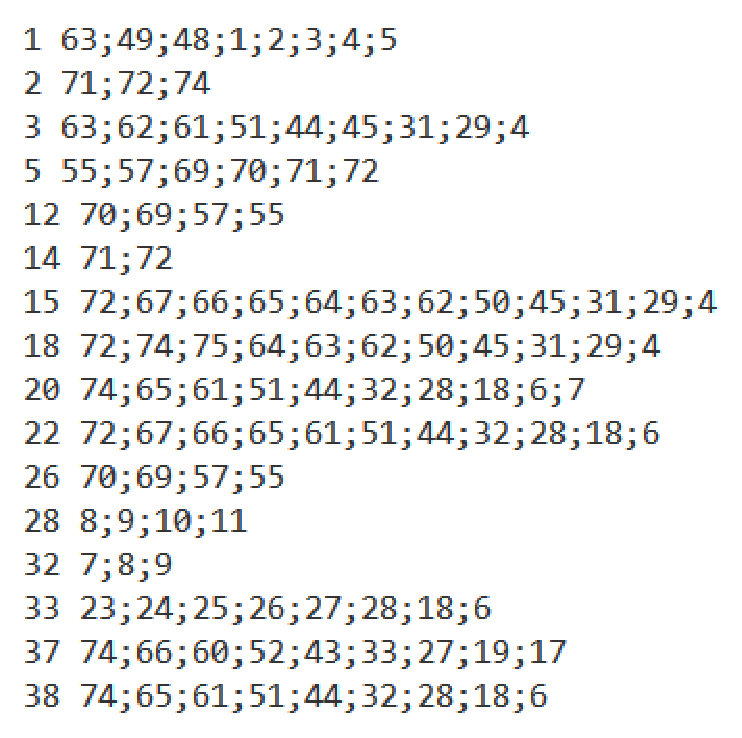
\includegraphics[height=1.6in, width=1.5in]{bus.eps}
\label{subfig:route}
}
\subfigure[]{
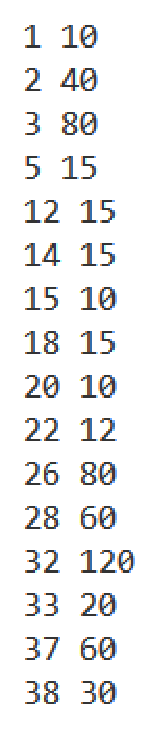
\includegraphics[height=1.6in, width=0.3in]{interval.eps}
\label{subfig:interval}
}
\caption{Figure~\ref{subfig:route} is part of the bus route information (totally 124 routes), where the entries for each bus are its route number and the stops (in the selected area) on its route; Figure~\ref{subfig:interval} is part of the bus interval information, where the
number in the second entry is the departure interval of the corresponding route.}
\label{fig:bus}
\end{figure}

\section{Agents}

In our scenario, only two kinds of agents are involved in the simulation framework to simply the over-complex world we want to model. 
The following sections show how we assume them and model them:

\subsection{Buses}
In our task, the buses' behavior is simplify to listen to the orders from a centralized bus manager, whose work is scheduling the bus intervals and manage the routes. 
This bus manager plays the pivot role in our simulation. 
Since that all buses are issued directly by the bus manager, the bus manager must to maintain a policy (or a kind of configuration) to specify what task should be done now or how a task is been done.
Rather than running by its own internal will but by the guide from the centralized bus manager, the buses are sort of single agent system rather an multi-agent one in which usually the agents involved is more than two. 
However, even though the buses are run by a single agent system, it proves to be reasonable assumption because of the nature of buses is obeying the order (or a predefined route and time interval) rather than act freely even under the bus driver's control.
More specifically, the bus will have several parameter resources to refer before it starts to move to the next iteration. 
They are: 
\begin{itemize}
\item The route information that needs to follow from the bus manager. 
\item The start command sends from the bus manager. If a start command is sent to the bus, the bus will start its journey.
\item The bus interval sent also from the manager, which specifies how many minutes should send a bus out.
\item The traffic information encoded in the edges of the map graph.
\end{itemize}
The bus behavior will then be:
\begin{itemize}
\item It will look up the traffic information in the graph to decide its current speed at each iteration.
\item After the run of each move, if the bus passes a node, the bus will stop in the node if the node is one of the schedule stop handed from the bus manager.
\item If the bus reaches the end of the scheduled route, the bus will turn around and go back to the beginning of the route.
\item After the round trip route is finished, the bus will eliminate from the simulated world. All the necessary statistics will be collect to compute some indicator digits that help us to judge the performance.
\end{itemize}


\subsection{Clients}
At each iteration, client agents are generated on a given node and a given destination node.
The number of clients generated on a particular node is decided by the type of scenario we want to model, which will be explained more detailed in the following sections.
Furthermore, in order to reduce the computational cost, the clients' behaviors are assumed to always greedy in a global fashion.
A detailed explanation is show as follows:
\begin{itemize}
\item If a client is at a bus stop, it first compares all the buses stopping at this bus stop.
\item The client will then choose a bus whose one of the next-N stops will take him to the nearest node to his target destination. N is a positive integer. 
\item Then he will get on the chosen bus until the next stop is reached and repeat the process again.
\item Otherwise, the client will wait for the chosen bus until it comes into the stop.
\end{itemize}
At first glance, although greedy algorithm might be not that intuitive to us (or as least can only apply to partial group of people but not at all ),
we believe it can still reflect some interesting facts we want by the simplified simulation.


\section{Simulation}
In this section, we first introduce how we assume our environments how we run our simulations on the predefined environments.
Three scenarios to mimic the real world behavior under different time situations  and three different policies of bus agents are taken into consideration.
Last but not least, the experiment results, analysis, and discussion regarding to the results are presented at the end of this section.

\subsection{Environment Settings}
In our simulations, each iteration in the simulated world is one minute in the real world. We use a small time span for each iteration to mimic the continuous real environment dynamics as like as possible.
Three bus policies are take into consideration:
\begin{description}
\item[Original:] The current bus routes in operation in which the data is collected manually from internet.
\item[Chessboard:] The main policy that we want to compared with. A chessboard-like bus route configuration.
\item[All-pair:] A funny example we do in our experiments. We have a bus for each of the edges in the map. Each bus is only run on the give edge.
\end{description}
The virtual buses and clients take actions alternately at every minute/iteration.
We run 10000 minutes/iterations for every three real world scenarios and three different bus policy configurations.
We use three types of scenarios, they are: 
\begin{description}
\item [Off-peak time:] Under this scenario, the flow of people are assumed to be under the assumption of random walk theorem, the average flow of people from node to node is zero. In this case, the number of clients generating from a particular node $i$ is draw from a Gaussian distribution $N_{i}^{(o)} \sim Gauss(\mu^{(o)},\sigma^{(o)})$ with mean $\mu^{(o)}$ equal to 1.2 and variance $\sigma^{(o)}$ equal to 0.5.
\item [Morning rush hours:] This scenario tries to model the rush hours during each morning where people comes from the outskirts of the city. The only difference between it and the off-peak time is that the number of client generated from the verge node $v$ is draw from a Gaussian distribution $N_{v}^{(m)} \sim Gauss(\mu^{(m)},\sigma^{(m)})$ with mean $\mu^{(m)}$ equal to three times of other nodes 3.6.
\item [Evening rush hours:] This scenario tries to model the rush hours during each evening where people goes back to the outskirts of the city from inside. The only difference between it and the off-peak time is that the number of client generated from the non-verge node $n-v$ is draw from a Gaussian distribution $N_{n-v}^{(m)} \sim Gauss(\mu^{(m)},\sigma^{(m)})$ with mean $\mu^{(m)}$ equal to three times of other nodes 3.6.
\end{description} 

\subsection{Results}

\begin{figure}
\centering
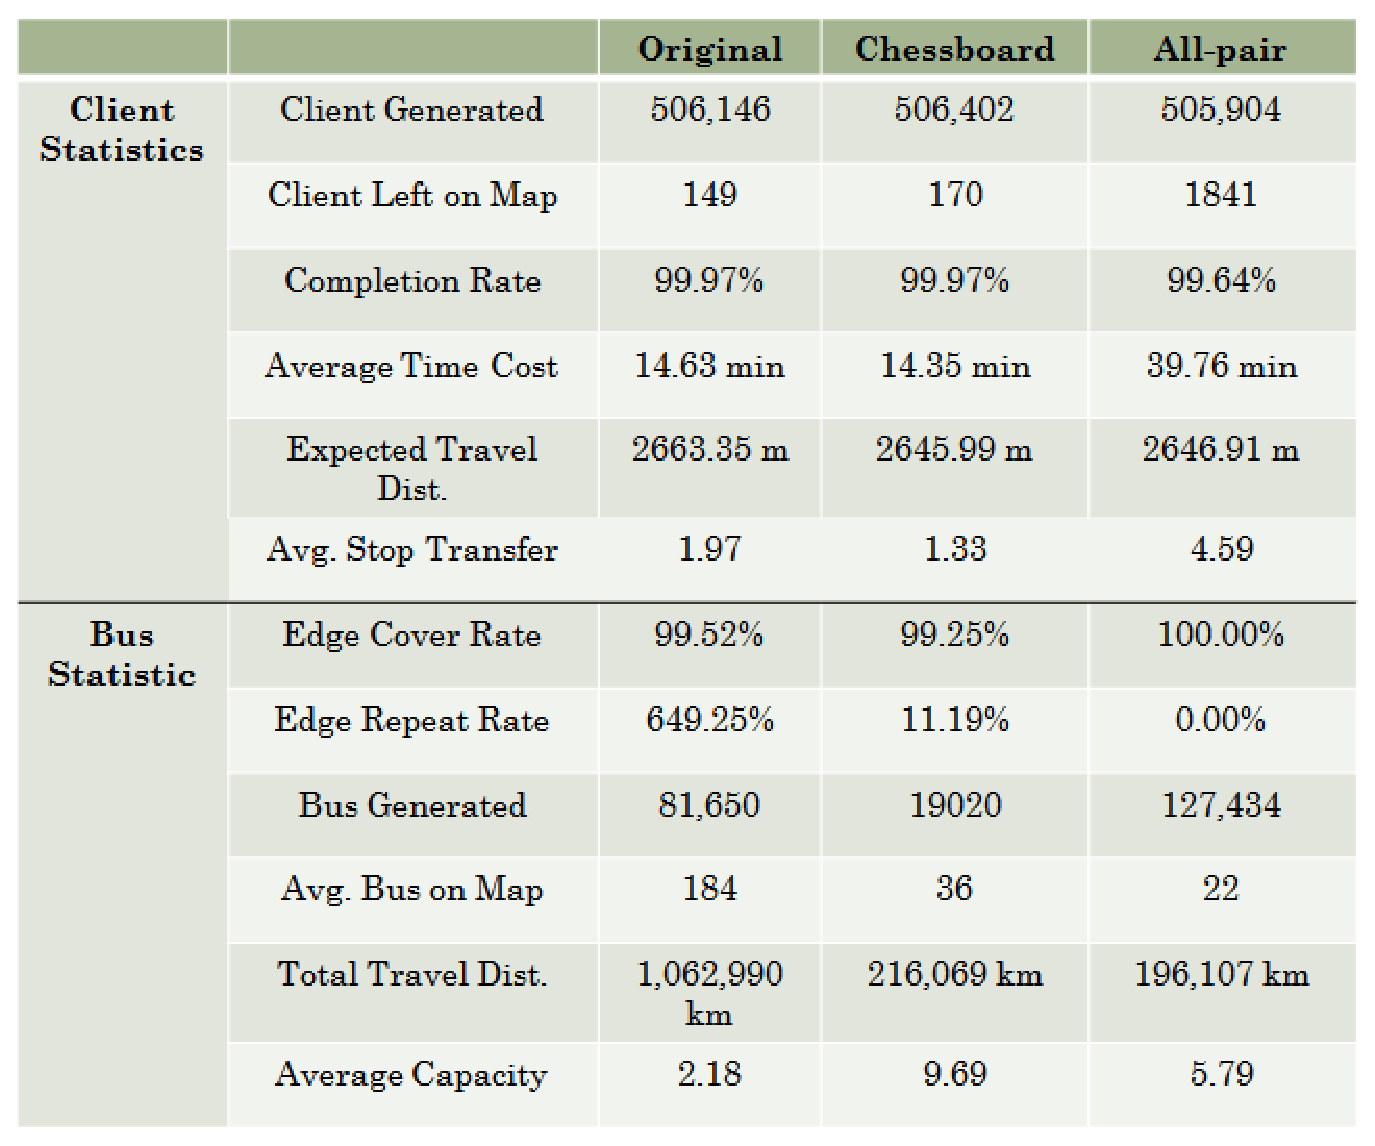
\includegraphics[height=2.5in, width=3.1in]{result1.eps}
\caption{Simulation under off-line scenario.}
\label{fig:exp1}
\end{figure}

\begin{figure}
\centering
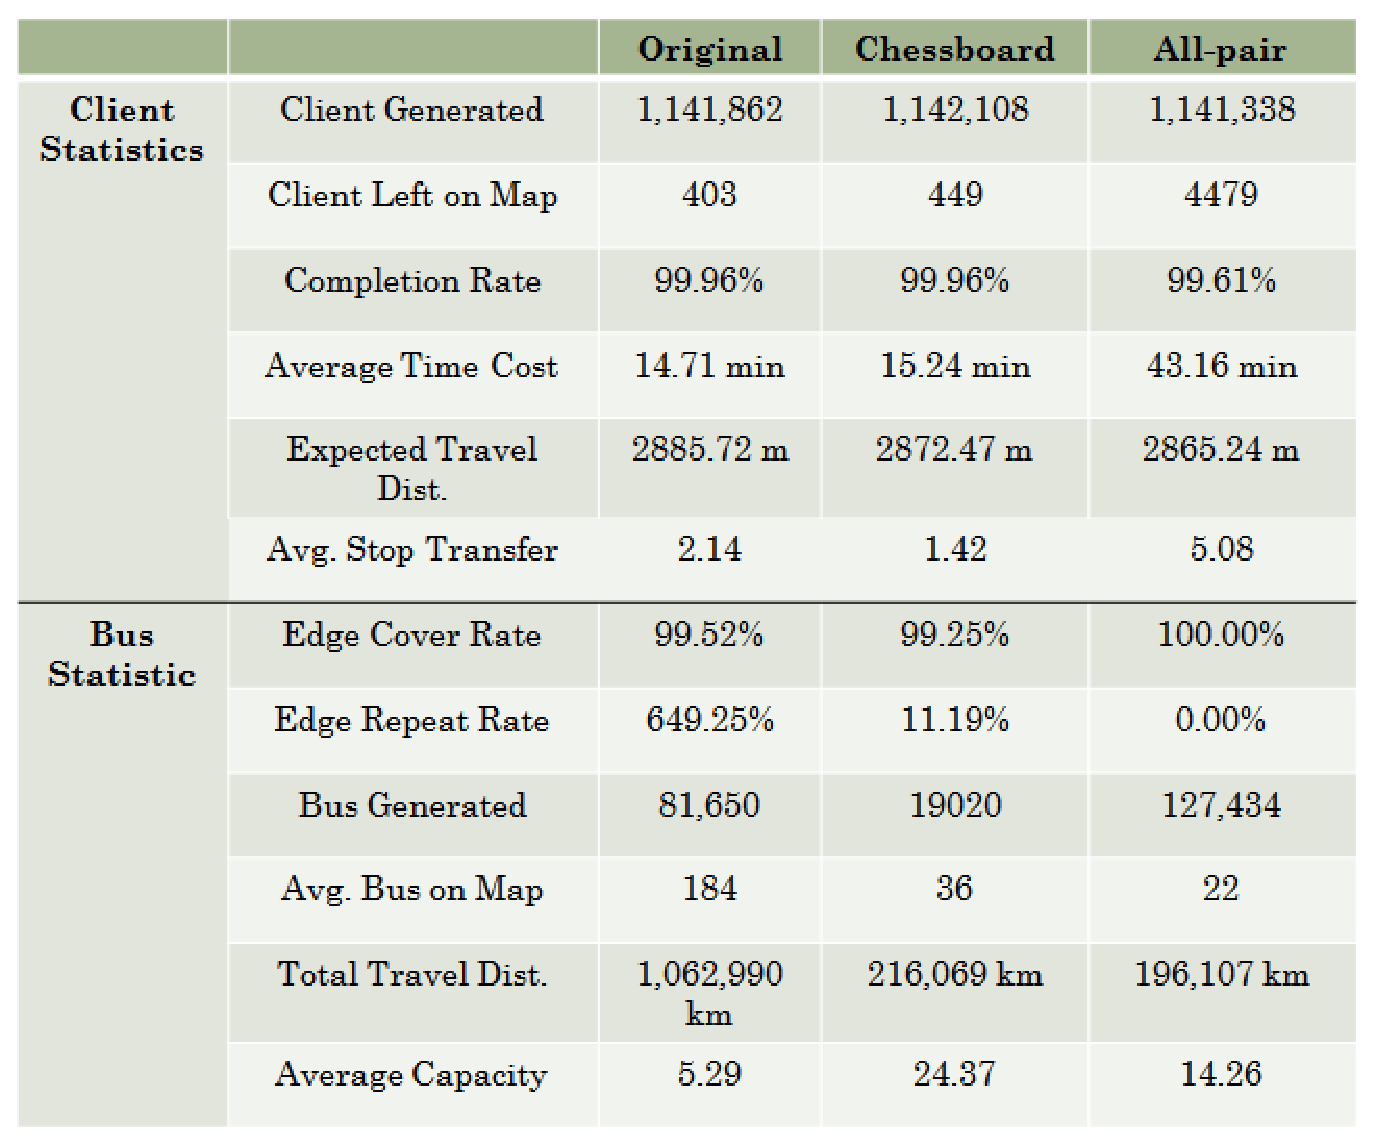
\includegraphics[height=2.5in, width=3.1in]{result2.eps}
\caption{Simulation under morning rush hour scenario.}
\label{fig:exp2}
\end{figure}

\begin{figure}
\centering
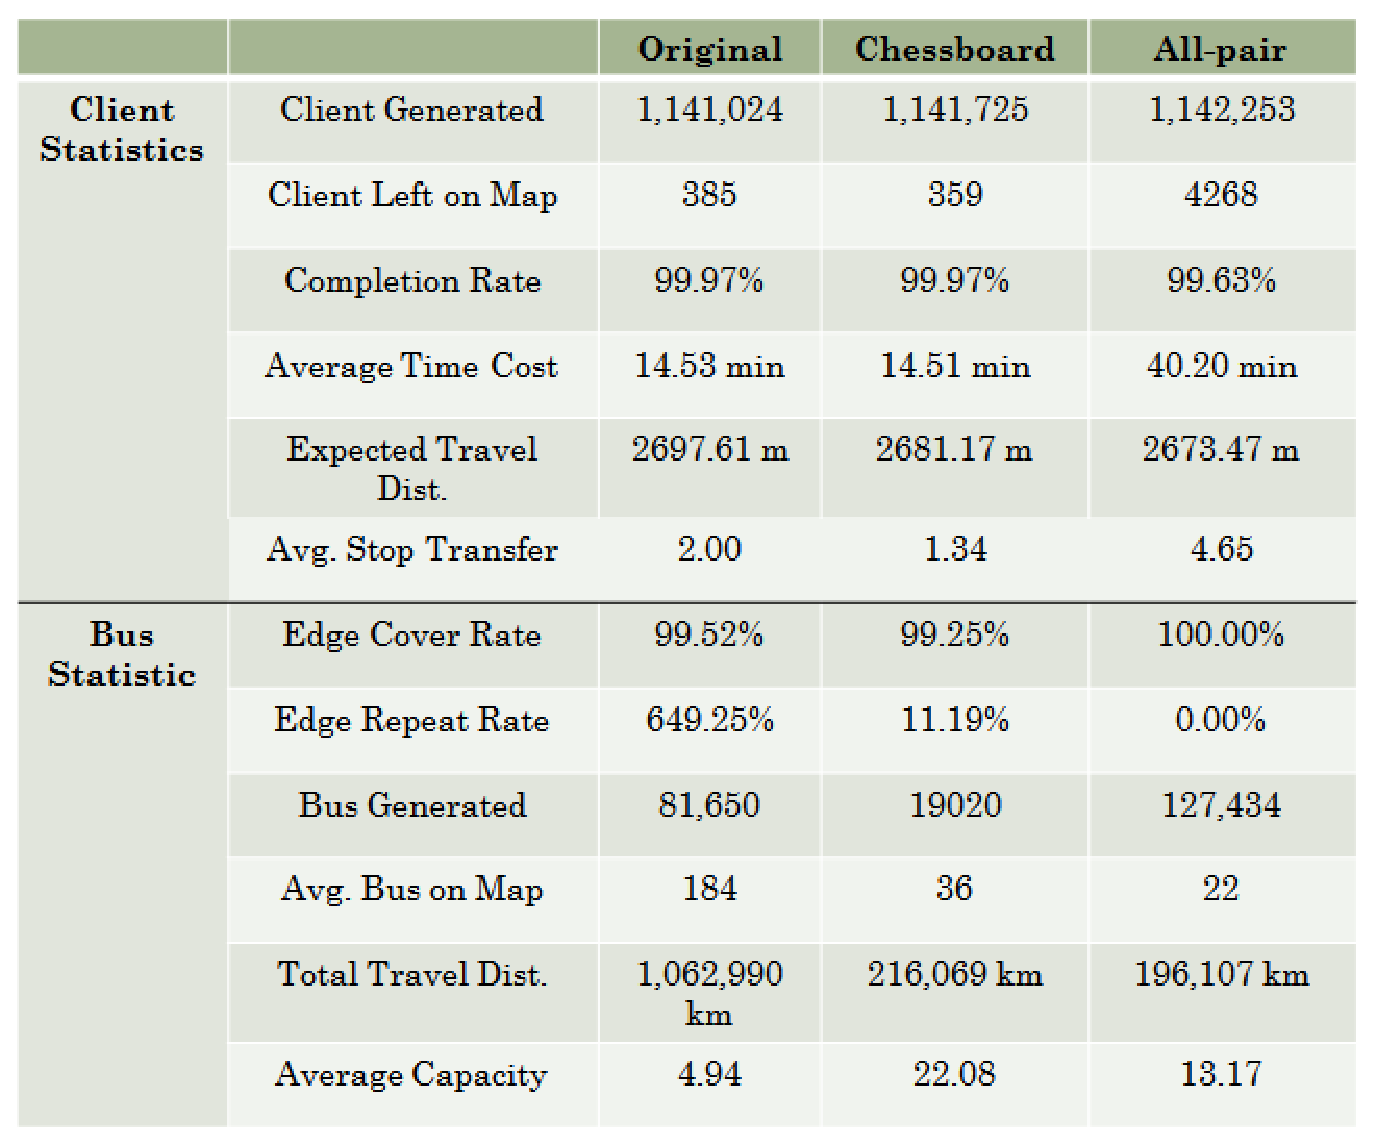
\includegraphics[height=2.5in, width=3.1in]{result3.eps}
\caption{Simulation under evening rush hour scenario.}
\label{fig:exp3}
\end{figure}


Fig.~\ref{fig:exp1}, Fig.~\ref{fig:exp2}, and Fig.~\ref{fig:exp3} shows our simulation result under three different bus policies when the scenario is off-peak, morning rush hour, evening rush hour respectively.

The client generated in three different scenarios are different since the gaussian mean is three times the number of Off-peak in verge nodes of Morning rush hour and Evening rush hour.
If we only look into the off-peak result in Fig.~\ref{fig:exp1}, you will discover that in client statistics, it is important to note that the average time cost is better for Original and Chessboard policy compared to All-pair policy but the Original and Chessboard is not so different. 
However, in average stop transfer, the Chessboard policy exhibits a better performance than the Original policy.
In bus statistics, the benefit of chessboard is very clear. 
The edge repeat rate is only 11.19\% compare to the extremely overlapped Original policy's 649.25\%.
The average bus left on the map is 36 for chessboard compared to 184 of original policy.
For the total travel distance, the chessboard is less thus save more energy compared to the original one.
And finally, for the average client capacity, the sparse capacity of original policy suggested that its overlapped nature makes the routes compete together and thus lower the overall efficiency of the system.
For Fig.~\ref{fig:exp2} and Fig.~\ref{fig:exp3}, the results shown also confirm to the Fig.~\ref{fig:exp1} result. 

\section{Conclusion}
We have discussed a problem about inefficient resource utilization of bus routes in Taipei city. 
Traditionally, the bus routes in Taipei city is full of detours, which makes the expected arrived time is far greater for a particular bus route. 
It also contains a lot of overlapped edges, which not only increase the number of buses need to be invested by the government and the bus companies but also decrease the utilization rate (average number of passengers) of a bus.
These are all indicators of the inefficiency resource utilization of real world.

With our model which cast the real world situation into a simpler world which only includes two agents: buses and clients.
The buses is then handled by a centralized bus manager whose responsibility is to schedule the bus under some predefined policies.
Clients are assumed greedy and thus also simply the computational cost.
The simulation is run under three different bus policies and three different scenarios.
The result suggested that chessboard, no matter in terms of the view of the client side but also the overall resource utilization side is far more efficient than the bus policy in operation now, as well as the all-pair poliscy.
Although in engineering's perspective, the chessboard policy does better than the current policy, the problem involves too many political and social issues underlines in the Taiwan local culture, the problem is not expected to be solved immediately in the near future but will progress toward a better direction gradually.
 


\end{document}